% !TEX encoding = UTF-8
%Koma article
\documentclass[fontsize=12pt,paper=letter,twoside]{scrartcl}

%Standard Pre-amble
\usepackage[top=4cm,bottom=4cm,left=3cm,right=3cm,asymmetric]{geometry}
%\geometry{landscape}                % Activate for for rotated page geometry
%\usepackage[parfill]{parskip}    % Begin paragraphs with an empty line rather than an indent
\usepackage[table,xcdraw]{xcolor}
\usepackage{graphicx}

\usepackage{amsmath}
\usepackage{amssymb}
\usepackage{epstopdf}
\DeclareGraphicsRule{.tif}{png}{.png}{`convert #1 `dirname #1`/`basename #1 .tif`.png}
% Listings needs package courier
\usepackage{listings} % Needs 
\usepackage{courier}

\usepackage[framemethod=TikZ]{mdframed}
\usepackage{url}

\usepackage{sty/bsymb} %% Event-B symbols
\usepackage{sty/eventB} %% REQ and ENV
\usepackage{sty/calculation}

%Maths
\usepackage{amssymb,amsmath}
\def\Fl{\mathbb{F}}
\def\Rl{\mathbb{R}}
\def\Nl{\mathbb{N}}
\def\Bl{\mathbb{B}}
\def\St{\mathbb{S}}
\newcommand{\ovr}{\upharpoonright}
\newcommand{\var}[1]{\textit{#1}}
%Useful definitions
\newcommand{\mv}[1]{\textit{m\_#1}}
\newcommand{\cv}[1]{\textit{c\_#1}}
\newcommand{\degree}[1]{^{\circ}\mathrm{#1}}
%\newcommand{\comment}[1]{{\footnotesize \quad\texttt{--}\textrm{#1}}}
\newcommand{\im}[1]{i\texttt{-\!#1}}

\usepackage[headsepline]{scrpage2}
\pagestyle{scrheadings}
\ihead[]{\small EECS4312 Report1}
\ohead[]{\small \thepage}
\cfoot[]{}
\ofoot[]{}


%%%%PVS environment%%%%%%%%%%%%%%%%%%%
\lstnewenvironment{pvs}[1][]
    {\lstset{#1,captionpos=b,language=pvs,
    mathescape=true,
    basicstyle=\small\ttfamily,
    numbers=none,
    frame=single,
    % numberstyle=\tiny\color{gray},
    % backgroundcolor=\color{lightgray},
    firstnumber=auto
    }}
    {}
 %%%%%%%%%%%%%%%%%%%%%%%%%%%%%%%%
 
%%%%Verbatim environment%%%%%%%%%%%%%%%%%%%
\lstnewenvironment{code}[1][]
    {\lstset{#1,captionpos=b,
    mathescape=true,
    basicstyle=\small\ttfamily,
    numbers=none,
    frame=single,
    % numberstyle=\tiny\color{gray},
    % backgroundcolor=\color{lightgray},
    firstnumber=auto
    }}
    {}

% \newenvironment{boxed}[1]
%    {\begin{center}
%    #1\\[1ex]
%    \begin{tabular}{|p{0.9\textwidth}|}
%    \hline\\
%    }
%    { 
%    \\\\\hline
%    \end{tabular} 
%    \end{center}
%    }
 %%%%%%%%%%%%%%%%%%%%%%%%%%%%%%%%
 
 %Text in a box
\newenvironment{textbox}
    {\begin{center}
    \begin{tabular}{|p{0.9\textwidth}|}
    \hline\\
    }
    { 
    \\\\\hline
    \end{tabular} 
    \end{center}
    }

\usepackage{hyperref}

%Highlight \hl{}
\usepackage{soul}

\usepackage{enumitem}
\newlist{mylist}{itemize}{1}
\setlist[mylist]{label=\textbullet,leftmargin=1cm,nosep}

\usepackage{multirow}

% Reduce space between figure and caption
%\usepackage{caption}
%\captionsetup[table]{font=small,skip=0pt}     %% Adjust here
%or equivalently 
\usepackage[font=small,skip=4pt]{caption}
%Useful definitions
%\newcommand{\mv}[1]{\textit{m\_#1}}
%\newcommand{\cv}[1]{\textit{c\_#1}}
%\newcommand{\degree}[1]{^{\circ}\mathrm{#1}}
%\newcommand{\comment}[1]{{\footnotesize \quad\texttt{--}\textrm{#1}}}

% Set the header
\ihead[]{\small EECS4312 Isolette Assignment}


%%%%%%%%%%%%Enter your names here%%%%%%%%
\author{\textbf{Juan Loja (lojag95@cse.yorku.ca)}
\and \textbf{Sadman Sakib Hasan (cse23152@cse.yorku.ca)}
}
%%%%%%%%%%%%%%%%%%%%%%%%%%%%%%%%

\date{\today} % Display a given date or no date

\begin{document}
\title{EECS4312 Isolette Assignment}
\maketitle

\noindent \textbf{Prism account used for submission}: cse23152@cse.yorku.ca

\begin {mdframed}
\textbf{\copyright This document is not for public distribution}. This document may only be used by EECS4312 students registered at York University. By downloading this document from the department, registered York students agree to keep this document (and all documents associated with assignments, projects or laboratories) private for their personal use, and may not communicate it to anyone else. 

Students must obey York regulations on academic honesty requiring that students do the work of the Lab on their own, and not cheat by sharing with others or using and/or submitting the work of others. If you use \textit{github} or similar repository for your work,  the repository must be private. Placing your work in the public domain infringes on academic integrity. Github offers unlimited private repositories to students: \url{https://education.github.com/pack}.

\end {mdframed}

\newpage

\vspace*{2in}
\begin{center}
\huge{\textbf{Requirements Document}:\\ Temperature control for an Isolette}
\end{center}

\bigskip\bigskip

\section*{Revisions}

%%%%%%%%%%%%Table of revisions%%%%%%%%
\begin{tabular}{|l|l|p{3in}|}
\hline
Date & Revision& Description \\ 
\hline
22 October  2017
& 1.0       
& Initial requirements document\\ 
\hline
\end{tabular}
%%%%%%%%%%%%%%%%%%%%%%%%%%%%%%%%

\newpage

%%%%%%%%%%%%%%%%%%%%%%%%%%%%%%%
\tableofcontents
\listoffigures
\listoftables
\newpage

%%%%Rest of your document goes here%%%%%%%%%%%%%%%%%%%

\section{System Overview}

The System Under Development (SUD) is a computer controller for the thermostat of an Isolette.\footnote{%
The image in Fig~\ref{fig:isolette} is from: \url{www.nufer-medical.ch}.}
An Isolette is an incubator for for an infant that provides controlled temperature, humidity and oxygen (Fig.~\ref{fig:isolette}). Isolettes are used extensively in Neonatal Intensive Care Units for the care of premature infants.

This requirements document is specifically for the control of temperature. The purpose of the Isolette computer controller is to maintain the air temperature of an Isolette within a desired range. It senses the current temperature of the Isolette and turns the heat source on and off to warm the air as needed. If the temperature falls too far below or rises too far above the desired temperature range, it activates an alarm to alert the nurse. The system allows the nurse to set the desired temperature range and to set the alarm temperature range outside the desired temperature range of which the alarm should be activated. This requirements documents follows the specification in \cite{REMH} (Appendix A) except where noted.

\begin{figure}[!htb]
\begin{center}
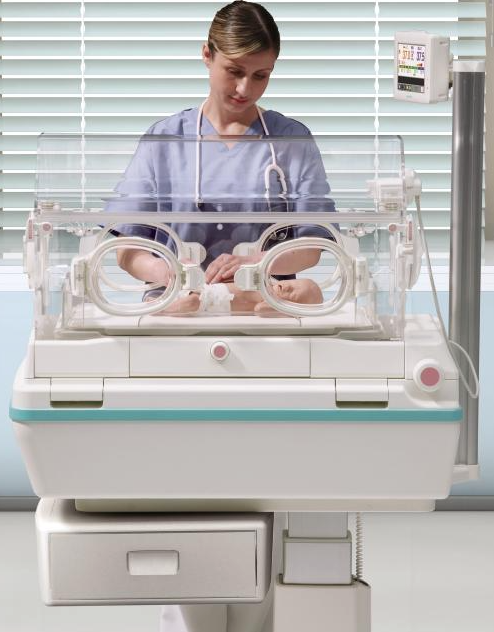
\includegraphics[width=.4\textwidth]{images/isolette.png}
\end{center}
\caption{Isolette}
\label{fig:isolette}
\end{figure}


Many babies have dies due to faulty incubators. There is thus a standard that manufacturers must satisfy. Modern incubators are equipped with alarms for air temperature, skin temperature, oxygen concentration and humidity. The alarms are both visual such as red warning lamps, and audio such as beep signals. Once measured measured values exceed permitted limits as well as when faults occur in sensors. For one such incident leading to death see ``Medical Devices: Use and Safety" shown in Fig.~\ref{fig:incubator}. 

\begin{figure}[!htb]
\begin{center}
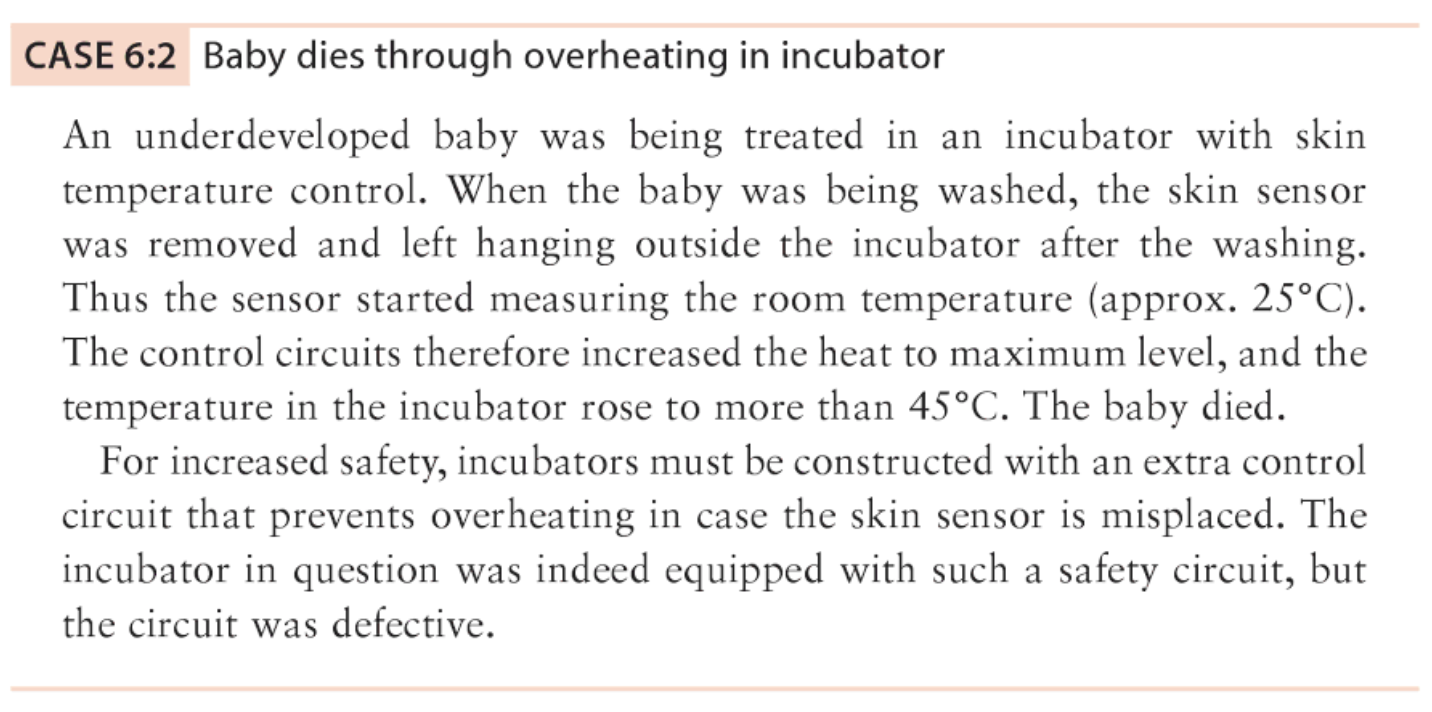
\includegraphics[width=.9\textwidth]{images/incubator.png}
\end{center}
\caption{Incubator Safety Problems \cite[p98]{JM2007}}
\label{fig:incubator}
\end{figure}

\section{Goals}

The high-level goals (G) of the system are:

\begin{mylist}
\item G1---The Infant should be kept at a safe and comfortable temperature.

\item G2---The Nurse should be warned if the Infant becomes too hot or too cold.

\item G3---The cost of manufacturing the computer controller for the thermostat should be as low as possible.
\end{mylist}


\newpage
\section{Context Diagram}

\begin{figure}[!htb]
\begin{center}
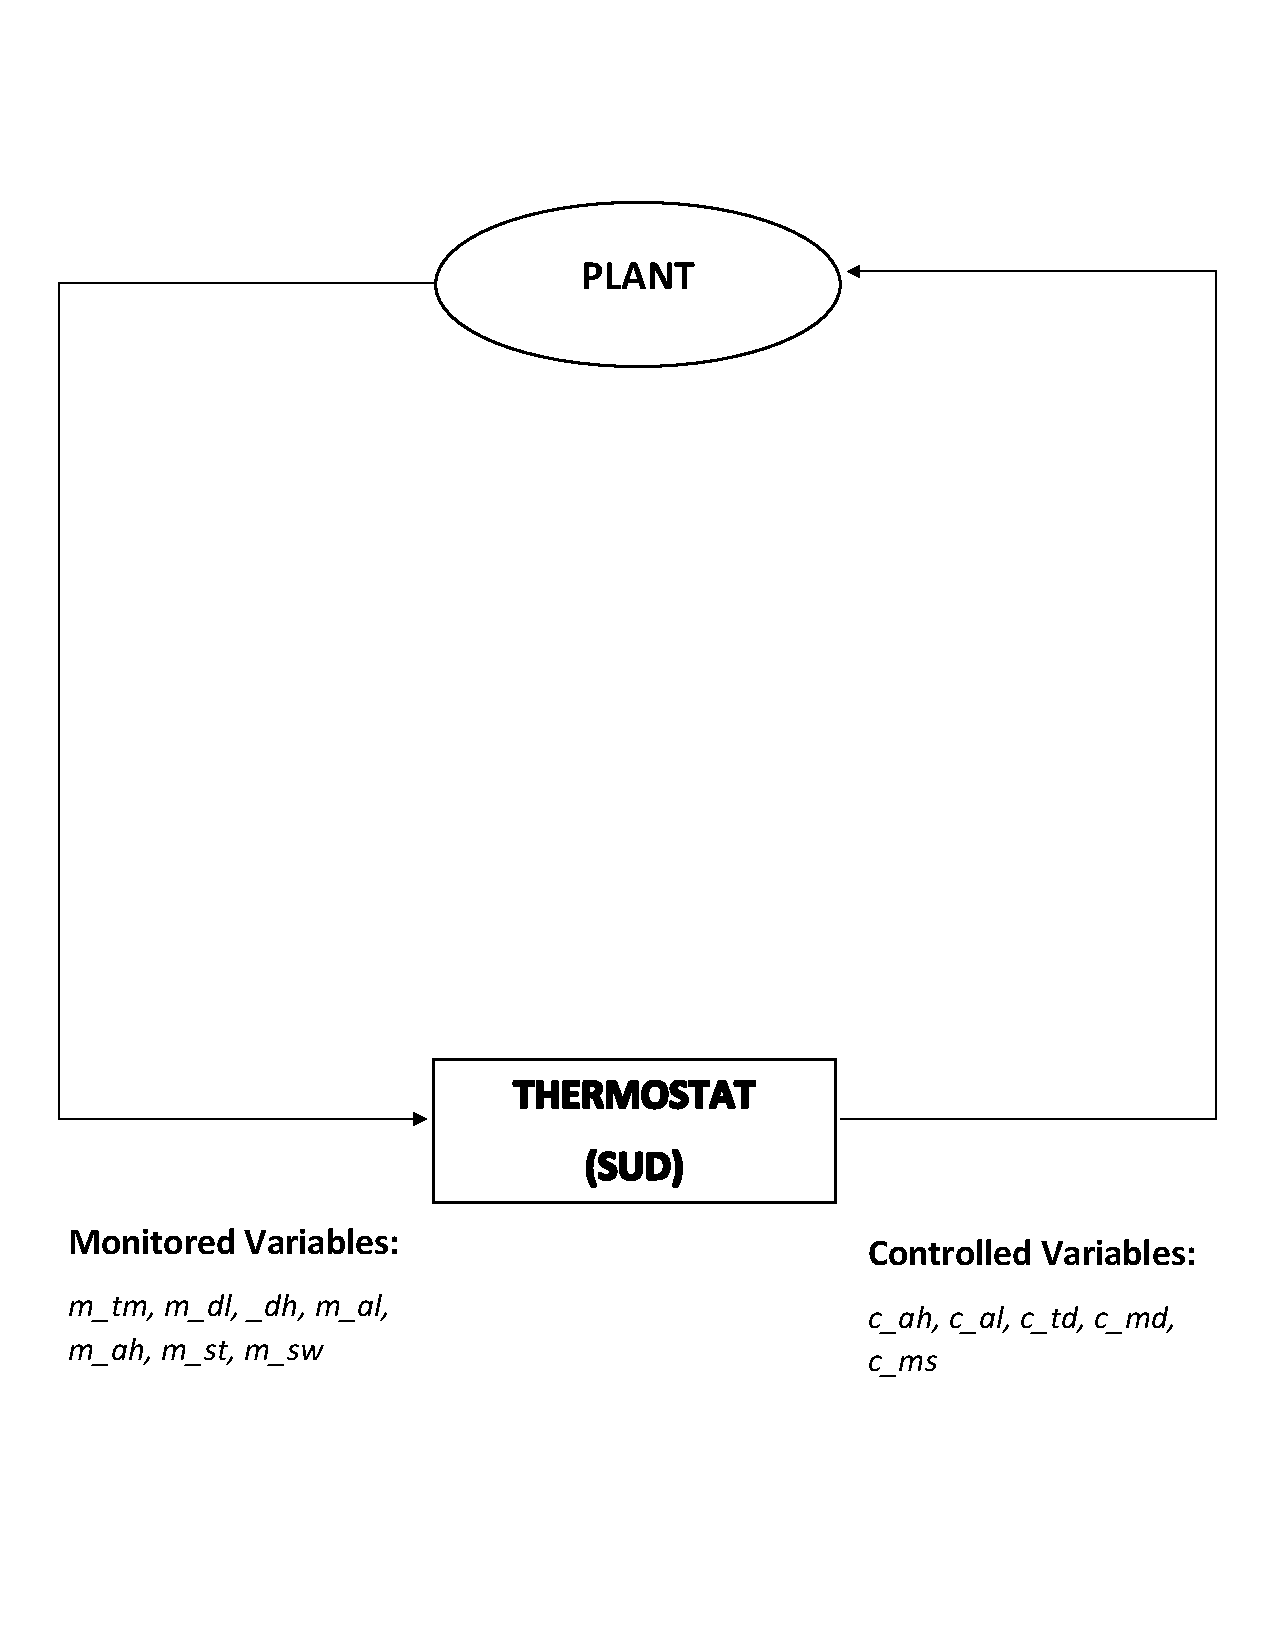
\includegraphics[width=.8\textwidth]{images/context-diagram.pdf}
\end{center}
\caption{Context diagram for the SUD}
\label{fig:context}
\end{figure}



\newpage
\section{Monitored Variables}

The monitored variables are a subset of those described in \cite{REMH}.\footnote{With some change of nomenclature. Monitored variables have an ``m'' prefix.} There is a single status variable \mv{st} that is \emph{invalid} whenever any one of the operator inputs or temperature sensor are in a failed state. Otherwise types and ranges are as in \cite{REMH}.

% Please add the following required packages to your document preamble:
% \usepackage[table,xcdraw]{xcolor}
% If you use beamer only pass "xcolor=table" option, i.e. \documentclass[xcolor=table]{beamer}
\begin{table}[h]
\begin{tabular}{|l|l|l|l|l|}
\hline
\cellcolor[HTML]{EFEFEF}Name & \cellcolor[HTML]{EFEFEF}Type & Range              & \cellcolor[HTML]{EFEFEF}Units & \cellcolor[HTML]{EFEFEF}Physical Interpretation                                       \\ \hline
\mv{tm}                      & $\Rl$                        &   $68 \upto 105$              &     $\degree{F}$                           & \begin{tabular}[c]{@{}l@{}}actual temperature of Isolette \\ air temperature from sensor\end{tabular} \\ \hline
\mv{dl}                      & $\intg$                      & $97 \upto 99$      & $\degree{F}$                   & \begin{tabular}[c]{@{}l@{}}desired lower temperature\\ set by operator\end{tabular}   \\ \hline
\mv{dh}                      & $\intg$                      &     $98 \upto 100$                            &    $\degree{F}$              & \begin{tabular}[c]{@{}l@{}}desired higher temperature\\ set by operator\end{tabular}  \\ \hline
\mv{al}                      & $\intg$                      &     $93 \upto 98$                            &    $\degree{F}$              & \begin{tabular}[c]{@{}l@{}}lower alarm temperature\\ set by operator\end{tabular}     \\ \hline
\mv{ah}                      & $\intg$                      &     $99 \upto 103$                         &   $\degree{F}$               & \begin{tabular}[c]{@{}l@{}}higher alarm temperature \\ set by operator\end{tabular}   \\ \hline
\mv{st}                      & Enumerated                   & \{valid, invalid\} &                               & \begin{tabular}[c]{@{}l@{}}status of sensor and \\ operator settings\end{tabular}     \\ \hline
\mv{sw}                      & Enumerated                   & \{on, off\}        &                               & switch set by operator                                                                \\ \hline
\end{tabular}
\caption{Monitored Variables}
\label{table:monitored}
\end{table}


\newpage
\section{Controlled Variables}

The controlled variables are a subset of those described in \cite{REMH}.\footnote{With some change of nomenclature. Controlled variables have a ``c'' prefix.} In addition, there is a mode display \cv{md} and a message display \cv{ms}.\footnote{The mode ``off'' is added to that of Fig.~A-4 in \cite{REMH}, and the mode transitions have been changed.}

% Please add the following required packages to your document preamble:
% \usepackage[table,xcdraw]{xcolor}
% If you use beamer only pass "xcolor=table" option, i.e. \documentclass[xcolor=table]{beamer}
\begin{table}[h]
\begin{tabular}{|l|l|l|l|l|}
\hline
\cellcolor[HTML]{EFEFEF}Name & \cellcolor[HTML]{EFEFEF}Type & Range                                                                    & \cellcolor[HTML]{EFEFEF}Units & \cellcolor[HTML]{EFEFEF}Physical Interpretation                                                         \\ \hline
\cv{hc}                      & Enumerated                   & \{on, off\}                                                              &                               & \begin{tabular}[c]{@{}l@{}}heat control: command to\\ turn heat source on or off\end{tabular}           \\ \hline
\cv{td}                      & $\intg$                      & $\{0\} \bunion \{68 \upto 105\}$                                         & $\degree{F}$                  & \begin{tabular}[c]{@{}l@{}}displayed temperature of Isolette\\ (zero when Isolette is off)\end{tabular} \\ \hline
\cv{al}                      & Enumerated                   & \{off, on\}                                                              &                               & sound alarm to call nurse                                                                               \\ \hline
\cv{md}                      & Enumerated                   & \begin{tabular}[c]{@{}l@{}}\{off, init, \\ normal, failed\}\end{tabular} &                               & \begin{tabular}[c]{@{}l@{}}mode of Isolette operation\\ (failed if $\mv{st} = invalid$)\end{tabular}    \\ \hline
\cv{ms}                      & Enumerated                   &                               \begin{tabular}[c]{@{}l@{}}\{ok, too\_hot\_alarm, \\ too\_cool\_alarm, warming\_up, \\ cooling\_down, system\_error\}\end{tabular}                 & & messages to display to nurse                                                                            \\ \hline
\end{tabular}
\caption {Controlled Variables}
\label{tbl:cv}
\end{table}

\newpage
\section{Mode Diagram}

\begin{figure}[!htb]
\begin{center}
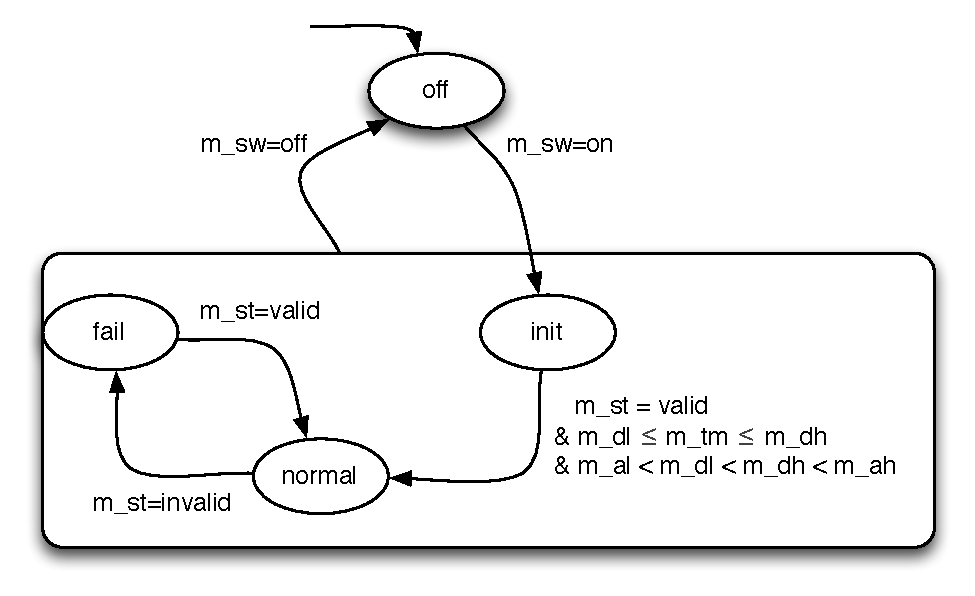
\includegraphics{images/mode-statechart.pdf}
\end{center}
\caption{Mode diagram for the states}
\label{fig:mode}
\end{figure}


\textbf{Rationale: } NEED RATIONALE HERE

%% Deactivate this to place your own work
%% !TEX root = ../sel-report.tex
\section{What is a good requirement?}

\begin{mdframed}[outerlinewidth=0.5,roundcorner=5pt]
A requirement is a separately verifiable contractual statement
stating a need of the customer
\end{mdframed}

\begin{itemize}

\item The customer has certain needs and goals. However, those needs are likely to be vague or incomplete. If you build an actual product, it is hard to see how you (or your customer) would check that the product you built satisfies the customer's needs. What is needed is a \textbf{precise requirements document}.

\item A precise requirements document describes everything necessary to produce a safe and correct system---one that fulfills the needs of the customer---nothing more. 

\item The requirements document must provide the software developer with \textbf{all} the information needed for the system to be built.

\item At the same time the specification must not over-constrain developers by venturing into design and implementation detail.

\item The requirements document thus specifies \emph{what} the system will do---not \emph{how} the system will do it!

\end{itemize}

\section{System Under Description}

Some stuff. Here is a png figure (see folder ``pics'')

\begin{figure}[htb]
\includegraphics[width=.4\textwidth]{pics/sud.png}
\includegraphics[width=.4\textwidth]{pics/sud.pdf}
\caption{PDF (right) displays better than jpeg or png (right)}
\label{fig:1}
\end{figure}

See Fig.~\ref{fig:1} for how to put an image in a figure environment. The ``htb'' says put the figure first here, then top of the page, then bottom, depending on layout algorithm. 

\section{R-descriptions and E-descriptions}
\reqm{ENV}
{Although it is physically possible for the trip and keypad commands to occur at the same time, the system is hardwired to respond sequentially (i.e. there is an arbitrary choice which one is dealt with first). Thus all signals arrive sequentially.}
{Refer to where your mathematical model uses this}
\label{E1}


\reqm{REQ}
{If the system is armed then a trip signal from the motion detector shall result in the siren being sounded.\\}
{Refer to mathematical model}
\label{R2}

\subsection{Subsection heading}

Other stuff with inline maths $p \limp q$ and 

\begin{equation}\label{eqn:1}
p \land q \lor r \limp z
\end{equation}

In (\ref{eqn:1}), we see how to write a formula.

Here is a verbatim environment with smaller text:

\begin{code}
=========================================
Use Case 1: uc1.txt: adding product types
=========================================
  report:      ok
  id:          0
  products:   
  stock:       
  orders:      
  carts:       
  order_state: 
->add_type("nuts")
  report:      ok
  id:          0
  products:    nuts
  ..
\end{code}

Here is some formatted PVS
\begin{pvs}
gate: THEORY
BEGIN
  p, q, r: bool
  not_gate(x: bool): bool = NOT x
  and_gate(x:bool, y:bool): bool = x AND y
  or_gate(x:bool, y:bool): bool = x OR y
  check1: CONJECTURE and_gate(p, not_gate(q)) => (p AND NOT q)
  check2: CONJECTURE and_gate(p, not_gate(q)) =  (p AND NOT q)

  circuit_implementation(x:bool, y:bool): bool = 
    and_gate(
              (or_gate(  and_gate(x, not_gate(y))
                       , and_gate(x,y))
             , y))

   and_conjecture: CONJECTURE
     and_gate(p,q) = circuit_implementation(p,q)

   or_conjecture:  CONJECTURE
     or_gate(p,q)  = circuit_implementation(p,q)
END gate
\end{pvs}

\begin{textbox}
Some text
\end{textbox}

\subsection{Signum Function}
Let's start with a simple example. In mathematics, the sign function or signum  (from \emph{signum}, Latin for ``sign") function $sgn(x)$ --- is a mathematical function that extracts the sign of a real number. In mathematical expressions the sign 

\begin{figure}[ht]
\begin{mdframed}[outerlinewidth=0.5,roundcorner=5pt]
\begin{minipage}{.4\textwidth}
\[sgn(x:\Rl) =
\begin{cases}
-1, &\text{if $x < 0$;}\\
0, &\text{if $x=0$;}\\
1, &\text{if $x >0$.}
\end{cases}\]
\end{minipage}
\qquad\qquad\qquad
\begin{minipage}{.5\textwidth}
\begin{tabular}{|l|l|}
\hline
        & $sgn(x)$ \\ \hline
$x < 0$ & -1     \\ \hline
$x = 0$ & 0      \\ \hline
$x > 0$ & 1      \\ \hline
\end{tabular}
\end{minipage}
\end{mdframed}
\caption{\small (a) Standard mathematical definition of $sgn(x)$. (b) Function table definition}
\end{figure}

The normal mathematical definition and the table layout are identical in meaning. However, the table layout is easier on the reader. Note that both description methods are \textbf{complete} and \textbf{disjoint}. 

\subsection*{Completeness}
The description of $sgn$ is complete because the function is defined for all possible inputs $x\in \Rl$. 

\subsection*{Disjointness}
The description is disjoint because each row in the table describes a case that is independent of the other rows --- hence avoiding inconsistencies 
--- where the same condition triggers different (and possibly contradictory) behaviours. 

For example, in a computer controlling a robot, we would not want the press of a \emph{move} button to signall to a robot to move right and move left at the same time.

The listing below shows how to describe the function in PVS.\footnote{%
See \url{https://wiki.eecs.yorku.ca/project/sel-students/p:tutorials:pvs:start}.}

 \section{Bibliography}
 
 See this \cite{Lamsweerde09}, this\ cite{GS93} and this \cite{Spivey92}. Run bibtex and then latex three times. 
\bibliographystyle{plain}
\bibliography{ref}

\newpage
\section{R-Descriptions}

We have already elicited the following R-descriptions.

\rdescription
{The \emph{controller} shall operate in one of four modes: \emph{off}, \emph{init}, \emph{normal} and \emph{fail}.\\}
{See statechart in Fig.~\ref{fig:sc}.}
\label{R1}

\rdescription
{In the \emph{normal} mode, the temperature controller shall maintain current temperature inside the Isolette within a set temperature range (the \emph{desired} range).\\}
{The \emph{desired} temperature range is $\mv{dl} \upto \mv{dh}$. If the current temperature \mv{tm} is outside this range, the controller shall turn the heater on or off via the controlled variable \mv{hc} to maintain the desired state.\smallskip}
\label{R2}

\smallskip
\noindent \textbf{Rationale}: The \emph{desired temperature range} will be set by the nurse to the desired range based on the infant's weight and health. The controller shall maintain the current temperature within this range under normal operation.

The following relevant hazard was identified through the safety assessment process:
\begin{mylist}
\item \textbf{H1}: Prolonged exposure of Infant to unsafe heat or cold;
\item \emph{Classification}: catastrophic;
\item \emph{Probability}: $<10^{-9}$ per hour of operation.
\end{mylist}

\noindent To ensure that probability of hazard H1 is $10^{-9}$ per hour of operation, the following derived safety requirement shall apply to the Isolette controller: 

\rdescription
{In \emph{normal} mode, the controller shall activate an alarm whenever 

\begin{mylist}
\item the current temperature falls outside the \emph{alarm} temperature range (either through temperature fluctuation or a change in the alarm range by an operator), or
\item a failure is signalled in any of the input devices (temperature sensor and operator settings).
\end{mylist}~}
{The alarm temperature range is $\mv{al}\upto\mv{ah}$.

Monitored variable \mv{st} 
%in Table~\ref{fig:mv} 
shows ``invalid'' when any of the input signals fail.}
\label{R3}


\rdescription
{Once the alarm is activated, it becomes deactivated in one of two ways:
\begin{mylist}
\item The nurse turns off the Isolette;
\item The alarm has lasted for 10 seconds, and after 10 seconds or more the alarm conditions are removed.
\end{mylist}~\\}
{\hl{Refer to the relevant tables of monitored and/or controlled variables and function tables.}}
\label{R4}


On the next page, you must add the next three most important R-Descriptions. Provide a brief rationale for each R-Description. Include any remaining R-Descriptions in an appendix to this document. 

\newpage
\hl{Additional three R-Descriptions with brief rational (one page)}

%%%%%%%%%%%%%%%%%%%%%%%%%%%%%%
\newpage
\section{E-descriptions}
\edescription
{The current temperature received from the sensor is a a real number in the range $68.0$ to $105.0 \degree{F}$.\\}
{??}
\label{E1}

\reqm{ENV}
{The desired and alarm temperatures received from the operator are all in increments of $1 \degree{F}$.\\}
{\hl{Refer to the relevant tables of monitored and/or controlled variables and function tables.}}
\label{E2}

\hl{Provide the next 3 most important E-descriptions on this page. The the rest in the appendix.}
%%%%%%%%%%%%%%%%
\newpage
\section{Abstract variables needed for the Function Table}

\hl{If needed, provide abstract variables here. Otherwise, state that abstract variables are not needed.}



%%%%%%%%%%%%%%%%%%%%%%%%%%%%
\section{Function Tables}

Starting on the next page, provide one function table for each control variable (in Table~\ref{tbl:cv}). Each control variable should have its own sub-section heading and its own page.

\newpage
\subsection{Function Table for heat control: \cv{hc}}

\hl{Function table goes here on this page. Other function tables each on their own page}

%%%%%%%%%%%%%%%%%%%%%%%%%%%%
\newpage
\section{Validation}
\hl{To be Done.} 
Proof of completeness and disjointness and validation of the requirements using PVS.

Include the PVS sources in the appendix to this document but summarize the proofs here.

%%%%%%%%%%%
\newpage
\section{Use Cases}

See Section A2 of \cite{REMH} for some use cases. The use cases need to be adapted to the revised descriptions of the previous sections of this document.
\hl{Provide one Use Case (a) informally and (b) formally in PVS.}

%%%%%%%%%%%%%%%%%
\newpage
\section{Acceptance Tests}

In this section, the use cases have to be converted into precise acceptance tests (using the function table to describe pre/post conditions) to be run when the design and implementation are complete. \hl{Describe one acceptance test}

%%%%%%%%%%%%%%%%%
\newpage
\section{Traceability}

Matrix to show which acceptance tests passed, and which R-descriptions they checked. No need to do this for this assignment. 


\section{Glossary}

The definition of important terms is placed in this section. You are not required to complete this.
%%%%%%%%%%%%%%%%%%%%%%%%%%%%%%%%%%%%%
\bibliographystyle{plain}
\bibliography{ref}

\newpage
\appendix

\section{Appendix Title??}
\hl{Appendix goes here. PVS sample below. Format so that there is no line wrapping}

\begin{pvs}
alert: THEORY
BEGIN
  delta: posreal = 0.5 % TR = 0.5 seconds
  IMPORTING Time[delta]

  p:     [DTIME -> real]  % Pressure
  alarm: [DTIME -> bool]

  hi: real
END 	
\end{pvs}

\end{document}  